%%%%%%%%%%%%%%%%%%%%%%%%%%%%%%%%%%%%%%%%%%%%%%%%%%%%%%%%%%%%%%%%%%%%%%%%%%%%%%%%
% Author : Jakub Július Šmýkal, Tomas Polasek (template)
% Description : Seventh exercise in the Introduction to Game Development course.
%   It deals with the creation of a Game Design Document, presenting a short 
%   pitch for a potential game project.
%%%%%%%%%%%%%%%%%%%%%%%%%%%%%%%%%%%%%%%%%%%%%%%%%%%%%%%%%%%%%%%%%%%%%%%%%%%%%%%%

\documentclass[a4paper,10pt,slovak]{article}

\usepackage[left=2.50cm,right=2.50cm,top=1.50cm,bottom=2.50cm]{geometry}
\usepackage[utf8]{inputenc}
\usepackage[T1]{fontenc}

% Hyper-Text References
\usepackage{hyperref}
\hypersetup{colorlinks=true, urlcolor=blue}

% Drawing Images and Graphs
\usepackage{tikz}
\usepackage{pgfplots}

% Page Utilities
\usepackage{graphicx}

% Image Sub-Captions
\usepackage{subcaption}

\newcommand{\ph}[1]{\textit{[#1]}}

\title{%
Game Pitch Document%
}
\author{%
Jakub Július Šmýkal (xsmyka01)%
}
\date{}

\begin{document}

\maketitle
\thispagestyle{empty}

{%
\large

\begin{itemize}

\item[] \textbf{Title:} Top down racing game

\item[] \textbf{Genre:} Závodná hra

\item[] \textbf{Style:} 3D/Top down

\item[] \textbf{Platform:} Windows, Xbox, Playstation

\item[] \textbf{Market:} Mladý ľudia

\item[] \textbf{Elevator Pitch:} Postav si vlastné pretekárske auto a vyhraj!

\end{itemize}

}

\section*{\centering The Pitch}

\subsection*{Introduction}
Cieľom hráča by bolo účastniť sa závodov, rôznych disciplín a minihier pre viacerých hráčov z ktorých by hráč zarábal hernú menu. Túto hernú menu by mohol hráč potom využiť na rozšírenie svojej kolekcie vozidiel a na ich úpravu.

\subsection*{Background}
K nápadu na závodnú hru ma inšpirovala moja záľuba k autám a ostatné závodné hry ako art of rally, forza horizon, ktoré ma veľmi bavia, ale nemajú možnosť rozsiahlo modifikovať výzor áut, či už z rozpočtových alebo licenčných dôvodov.

\subsection*{Setting}
Kedže by sa jednalo o hru pre viacero hráčov tak by sa v hre nenachádzal žiadny príbeh. Avšak preteky by sa konali v rôznych častiach sveta. Týmto spôsobom by sa dalo do hry zakomponovať rôzne mestské, snežné, púštne či lesné mapy. Pre vytvorenie väčšej rozmanitosti by sa mohli vyskytovať v hre určité mapy aj viac krát, ale vždy s nejakými zmenami, ako napríklad iné ročné obdobie, alebo iné desaťročie, čomu by boli prispôsobené výzory objektov a prekážok nachádzajúcich sa na mape. Každé prostredie by inak vplývalo na chovanie auta. Hráči by tak museli svoje autá prispôsobovať tomu, či sa chystajú pretekať po cestách, v snehu, alebo cez polia.

\subsection*{Features}
Hra by bola založená na voľnosti hráča upravovať si svoje auto. Autá by sa dali kupovať iba ako prázdna karoséria, do ktorej by si potom hráči dosadili preferované súčiastky. Všetky súčiastky upravujúce výkon a správanie sa auta by sa dali zdieľať bez obmedzenia medzi všetkými autami. Iba kozmetické súčiastky by boli obmedzené na jeden konkrétny typ karosérie. V hre by sa nachádzali rôzne časovo obmedzené disciplíny, pomocou ktorých by hráči mohli získať exkluzívne súčiastky. Tie by boli výhradne kozmetické, aby hráči neboli znevýhodnení za to, že sa im nepodarilo zúčastniť sa disciplíny. Aby sa predišlo výtváraniu príliš výkonných áut, ktoré by ostatným hráčom pri hraní kazili zážitok z hry, by sa hry pre viacero hráčov odohrávali v určitých triedach. Tieto triedy by rozdelovali autá podľa ich výkonu, váhy a obratnosti tak, aby všetky autá v jednej triede boli navzájom konkurenice schopné.

\subsection*{Platform}
Ako platformu som sa rozhodol vybrať windows a konzole z toho dôvodu, že sú to jedny z najviac využívaných platforiem na hranie hier. Okrem toho sa na týchto platformách dá hrať hry pomocou ovládača, čo by bol preferovaný spôsob ovládanie takejto hry. Mobilné platformy som sa rozhodol vynechať z toho dôvodu, že vybratý pohľad kamery by výrazne znižoval zážitok z hry, kedy by boli všetky objekty na obrazovke veľmi malé alebo by nebol dostatočný výhľad hráča pred vozidlo.

\subsection*{Style}
\begin{figure}[h]
\centering

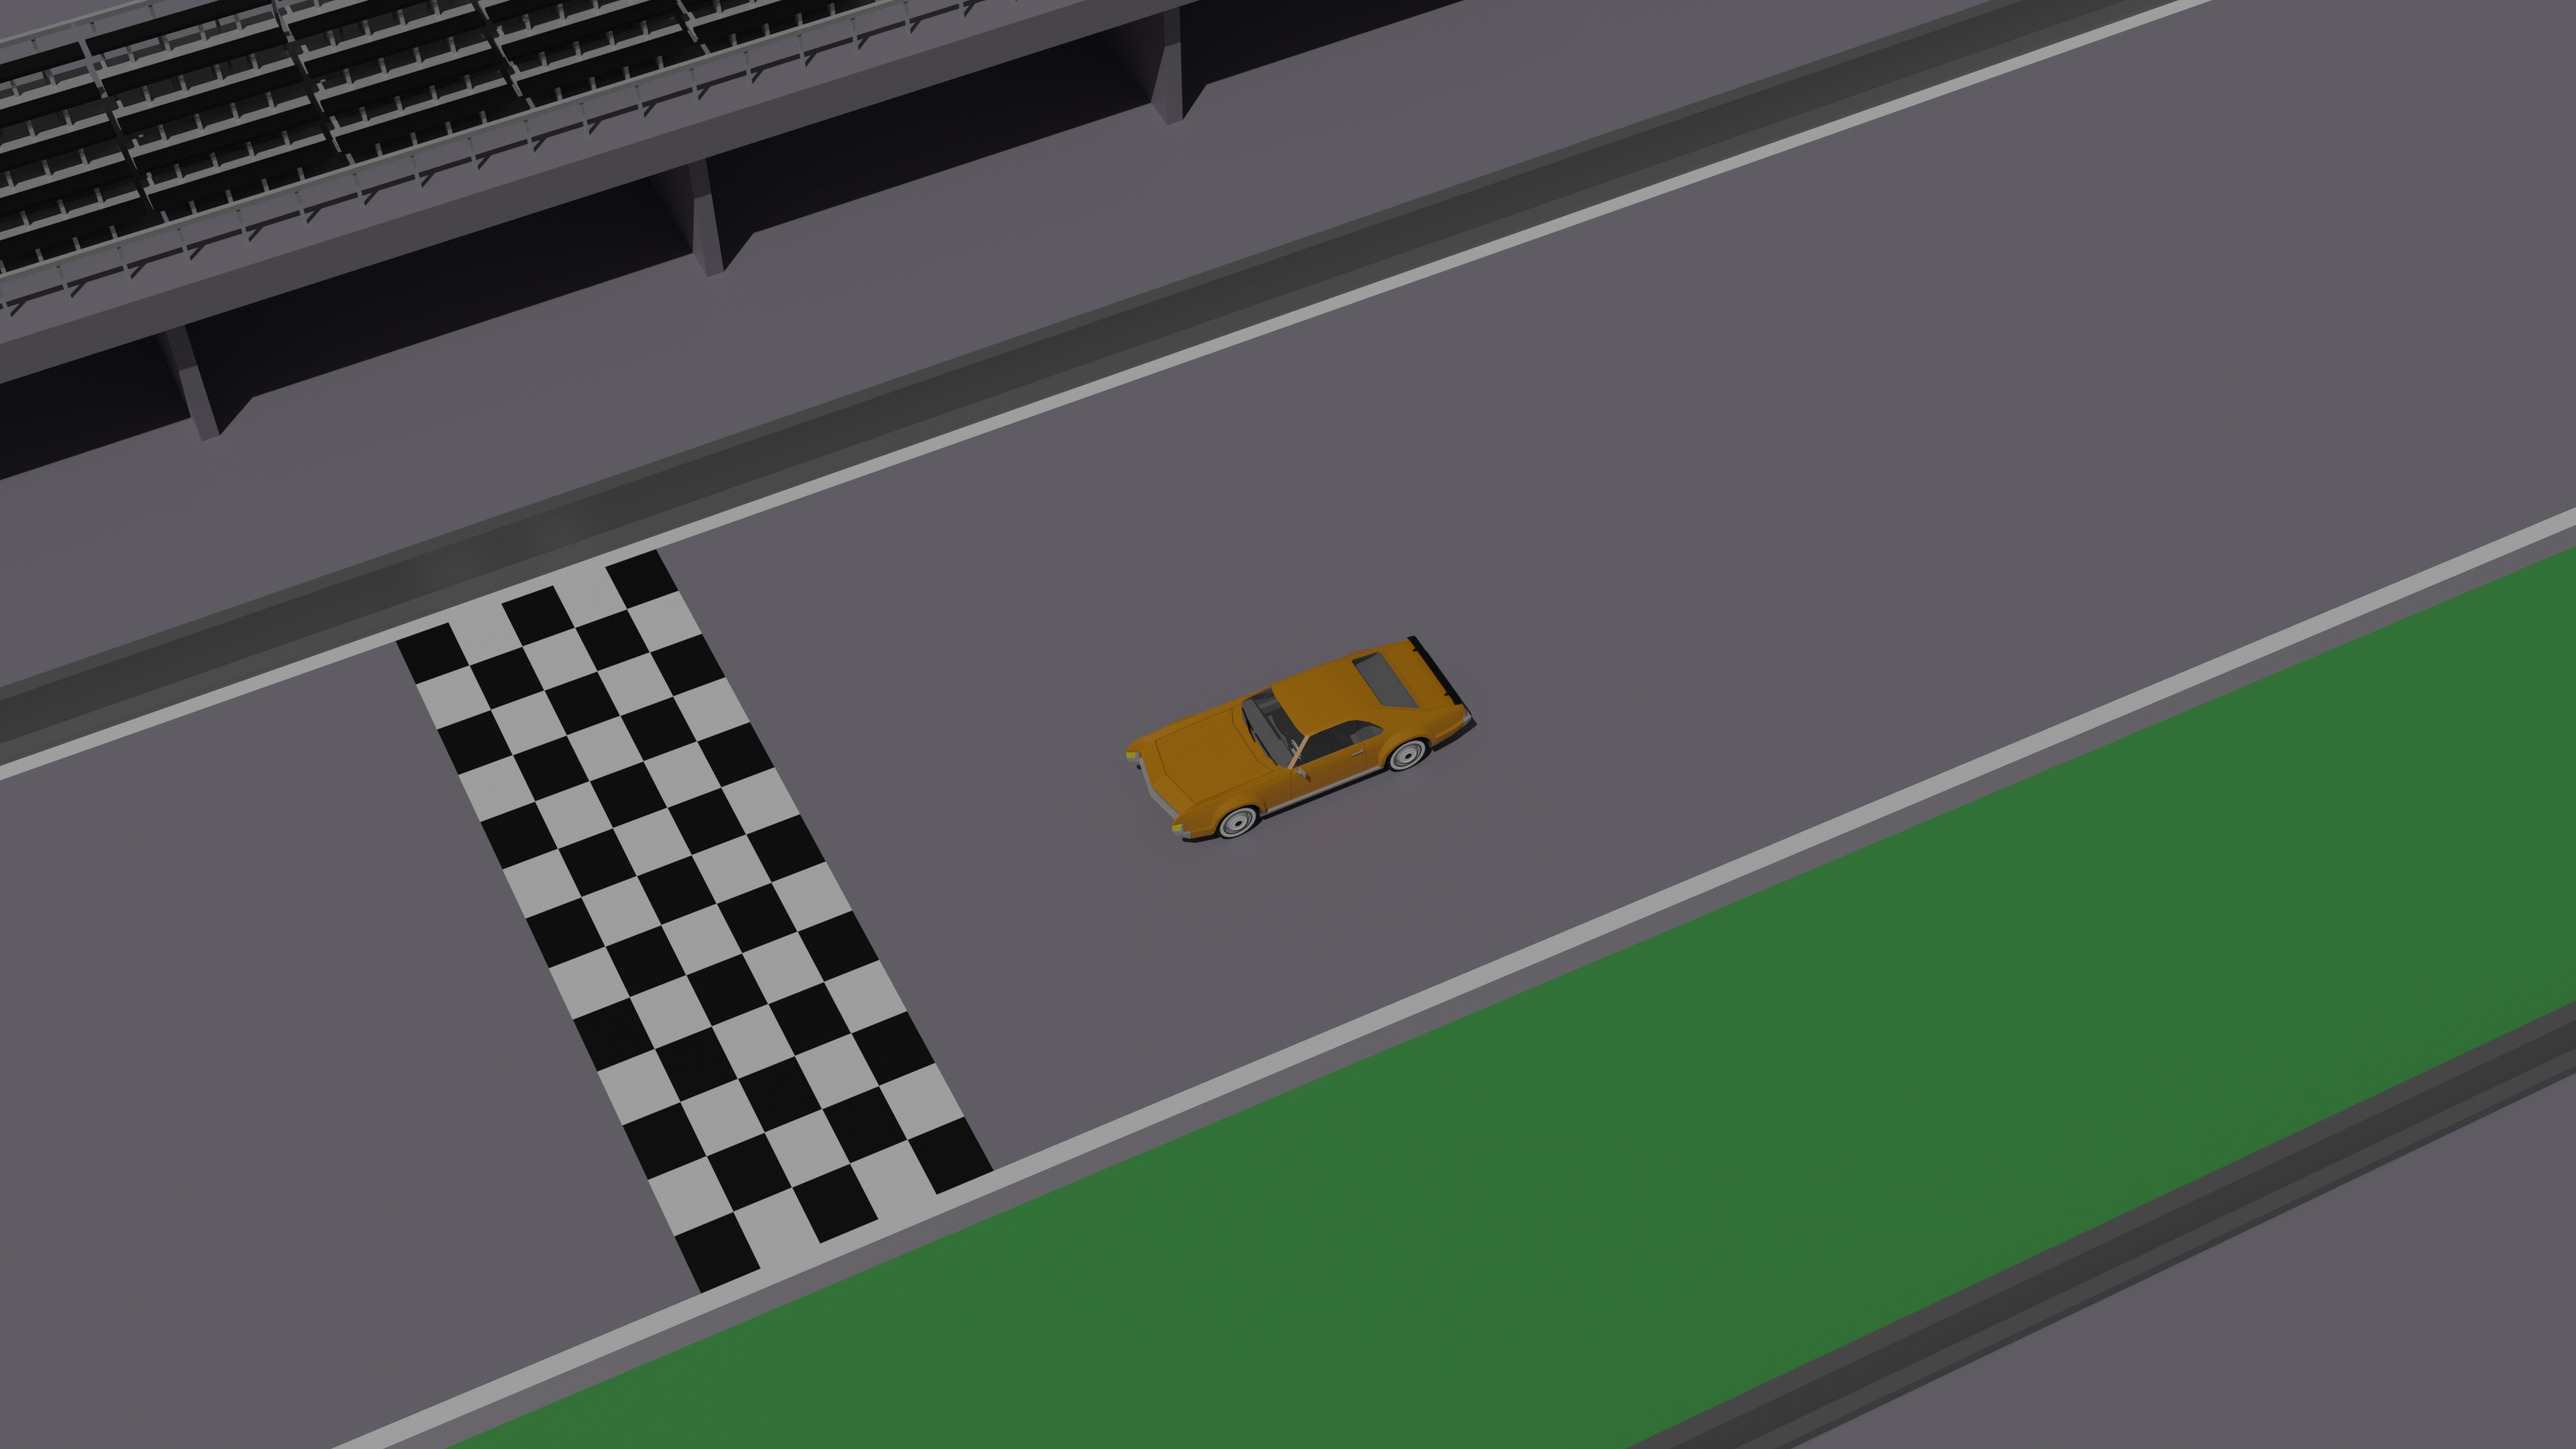
\includegraphics[width=\linewidth]{untitled.jpg}
\captionof{figure}{Render zobrazujúci možný výzor hry}
\label{Fig:render}

%
\end{figure}

\end{document}
